\section{Datensatz}
\label{sec:02_Datensatz}

Der Datensatz wurde mittels einer PiCamera (cite) in einem Zeitraum von 3 Wochen
aufgenommen. 
Die Größe des Datensatzes ist beliebig erweiterbar aber wurde aufgrund der
Zeitlichen einschränkung zur evaluation auf \num{4000} Fotos beschränkt. 

Desweiteren spielt die Zeit in der Die Daten aufgenommen werden eine wesentliche
Rolle.
Abhaengig der Jahreszeiten aendert sch die relative Häufigkeit in der die verschiedene
Wolkentypen aufgenommen werden koennen und somit in dem Datensatz repräsentiert sind. 
So sind zum Beispiel gut-Wetter Wolken viel stärker vertreten als die von
Regenwetter. 
Zu den elf Wolkenklassen die auch die Klasse keine Wolken einschließt zählt
ebenso eine 'schlechte Fotos' Klasse. 
Aufgrund von zufAlligen als auch zeitlichen Ereignissen werden Fotos produziert
anhand derer keine Wolekklassifikation vorgenommen werden kann.
Ein Beispiel dafür ist wenn eine Person das sichtfeld verdeckt oder es Nacht ist
und die Wolkendecke aufgrund fehlender belichtung nicht erkannt werden kann. 

\begin{wrapfigure}{l}{0.35\textwidth}
		\centering
		\vspace{-0.5cm}
		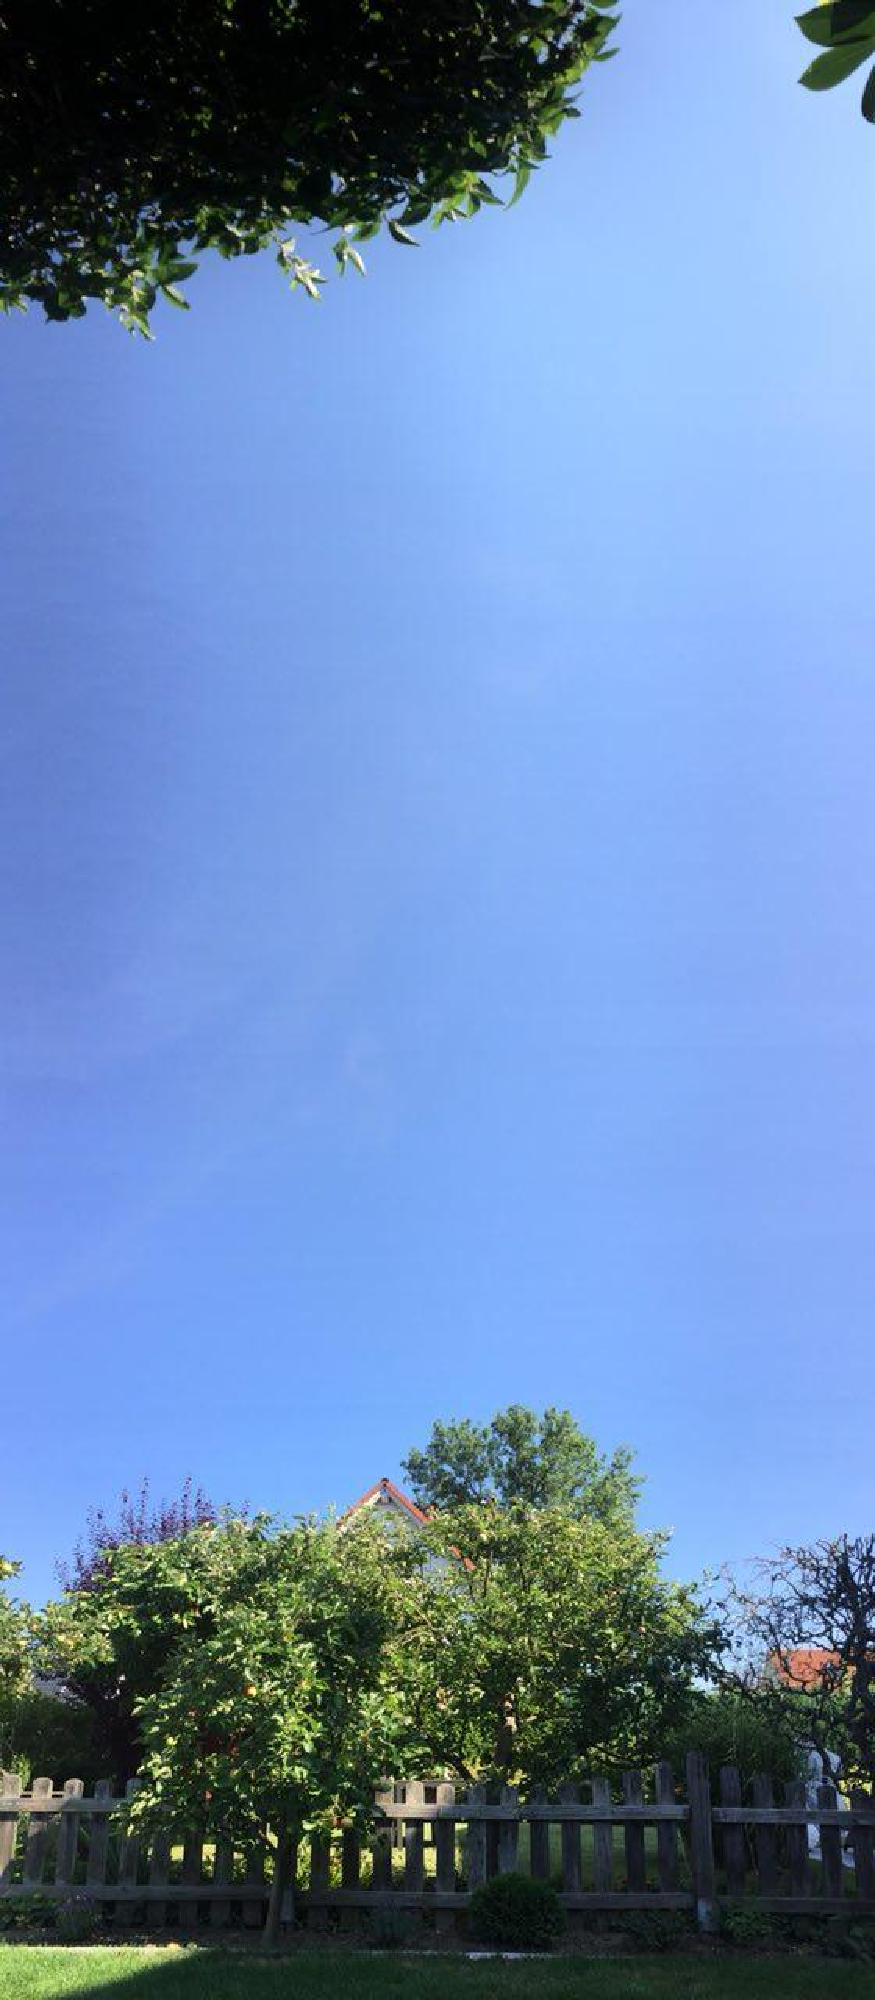
\includegraphics[width=0.3\textwidth]{./build/station_winkel.pdf}
		\caption{Wolkenausschnitt in Abhaengigkeit des Observationswinkel}
		\label{fig:theta}
		\vspace{-0.5cm}
\end{wrapfigure}
Die Wolkenfotos wurden an zwei voneinander unabhängigen Orten aufgenommen, wobei
Characteristiken der Aufnahmeorte auf den Bildern zu erkennen seien koennen.
Desweiteren stellte sich bei der Aufnahme des datensatzes heraus das eine
Ausrichtung der Kamera der Wetterstation nach Osten sinnvoll ist.
Dadruch laesst sich ein übermäßiges ausleuchten des Bildes durch die Sonne
verhindern, was den Kamerasensor schont.
Wie in Abbildung \ref{fig:theta} zu sehen, ist der Aufnahmewinkel $\theta$ 
entscheidend fuer die Klassifikation. 
Der Winkel $\theta$ gibt an, wie Steil die Kamera vom Boden richtung Wolken 
ausgerichtet ist.
Bei grossen Aufnahmewinkel ist nur ein kleinerer Teil der Wolkendecke zu sehen
als bei kleineren.
Bei diesen Ausschnitten stellt es sich als schwierig heraus sie der richtigen
klasse zuzuordnen da der Ausschnitt meist meherern Klassen zuzuordnen ist. 
Mit Grösseren Raumwinkeln lässt sich das Problem reduzieren, da dadurch ein
Größerer Teil der Wolkendecke observiert werden kann. 

Die aufgenommenen Daten besitzen a priori kein Label und sind auch nicht immer
eindeutig einer klasse zuzuordnen.
Anhand der im Anhang kurze Erklärung der unterschiedlichen Klassen wurden Sie
mittels eines eigen dafür programmierten
\href{https://telegram.me/weatherpi_bot}{\texttt{Telegram-Bot}} eingeteilt.
Mit hilfe von Freiwilliigen labelnern wurde jedes Foto des Datensatzes drei mal
klassifiziert und anschliessend per mehrheitsentscheid der Zielklasse zugeteilt.
Der Arbeitsaufwand wurde mit ca $\num{4000} \, \text{Bilder} \cdot \SI{1}{\hertz}$
abgeschätzt.
Aufgrund von aussetzern des Bots als auch ladezeit der Bilder konnte die Rate
auch nach einer Einarbeitungszeit nicht erreicht werden und die pro Bild benötigte Zeit entsprach schätzungsweise
\SI{15}{\second}
Bei der evulation der Modelle stellte sich heraus das bei Paralleler nutzung
sich eine interne Klassenvariable überschrieben wurde so das ein Großteil der
Klassifizierten Daten einer falschen finalen klasse zugeordenet wurden. 

Final steht ein Datensatz von \num{4000} Bildern welche in 10 Wolkenklassen und
eine Klasse mit schlechten Fotos aufgeteilt sind. Die Bilder besitzen eine Dimension 
von \texttt{(1024x768x3)} und liegen im \texttt{JPG}-Format vor.

\begin{figure}[h]
		\centering
		\begin{subfigure}[b]{0.31\textwidth}
		\begin{center}
				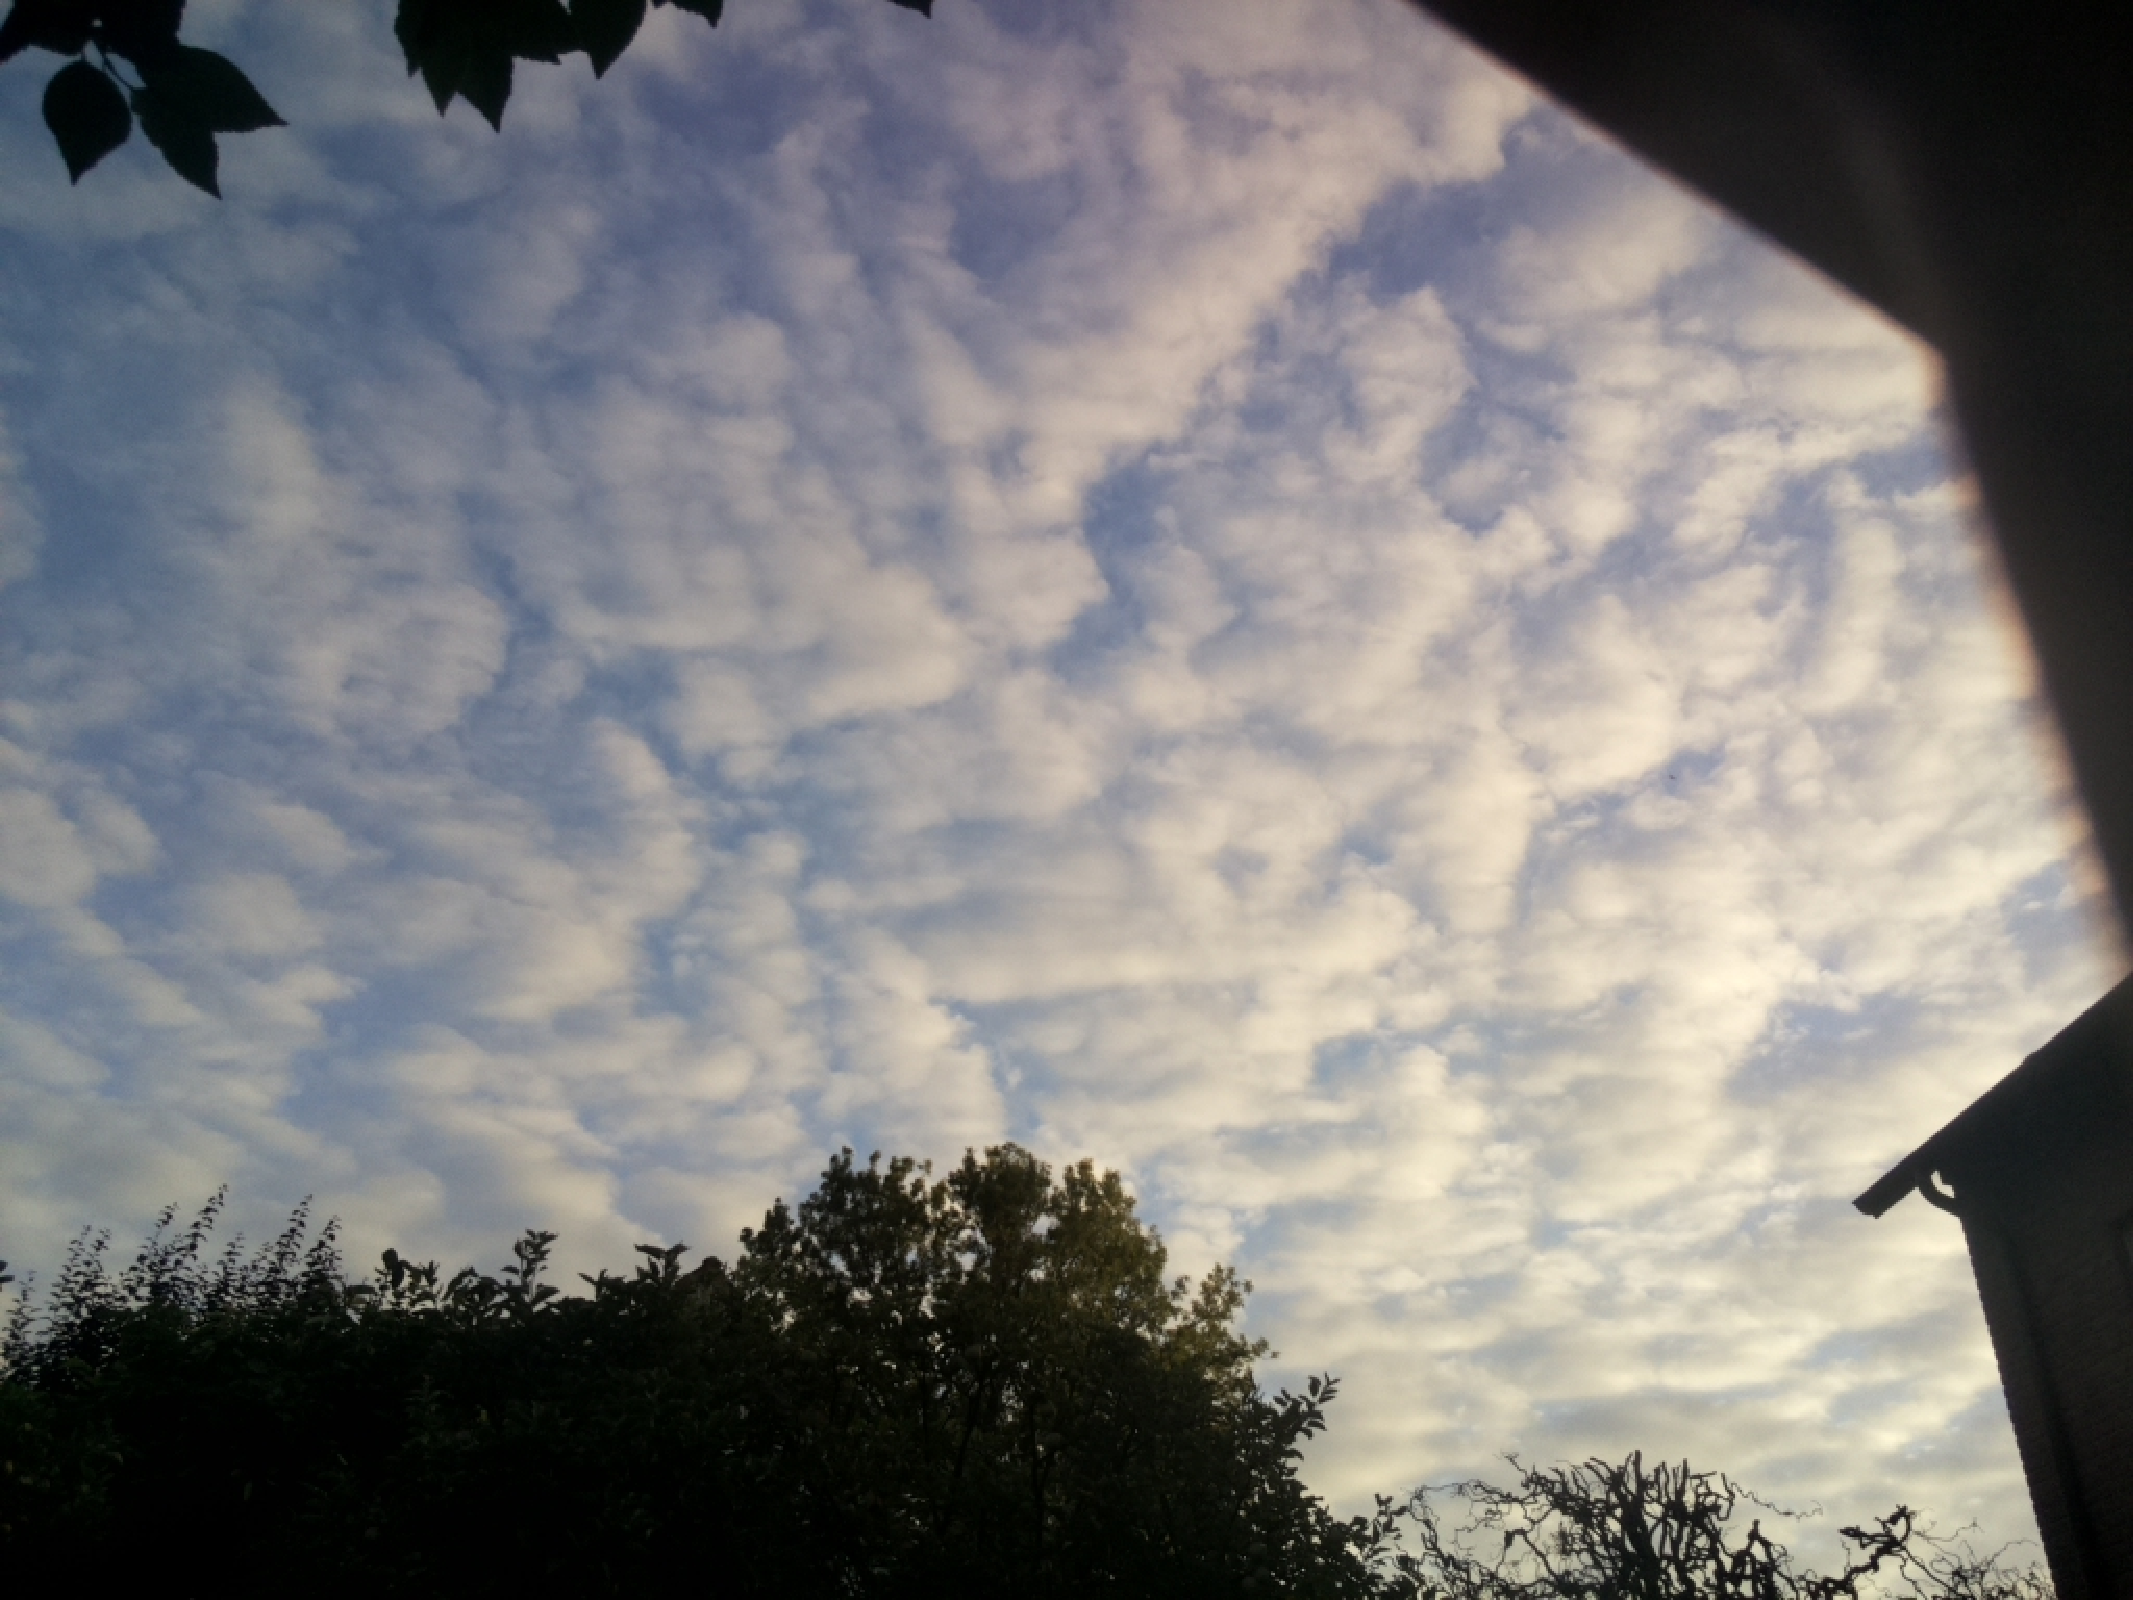
\includegraphics[width=\textwidth]{./pictures/cloudtypes/altocumulus.pdf}
		\end{center}
		\caption{Altocumulus}
		\label{fig:altostratus}
		\end{subfigure}
		\begin{subfigure}[b]{0.31\textwidth}
		\begin{center}
				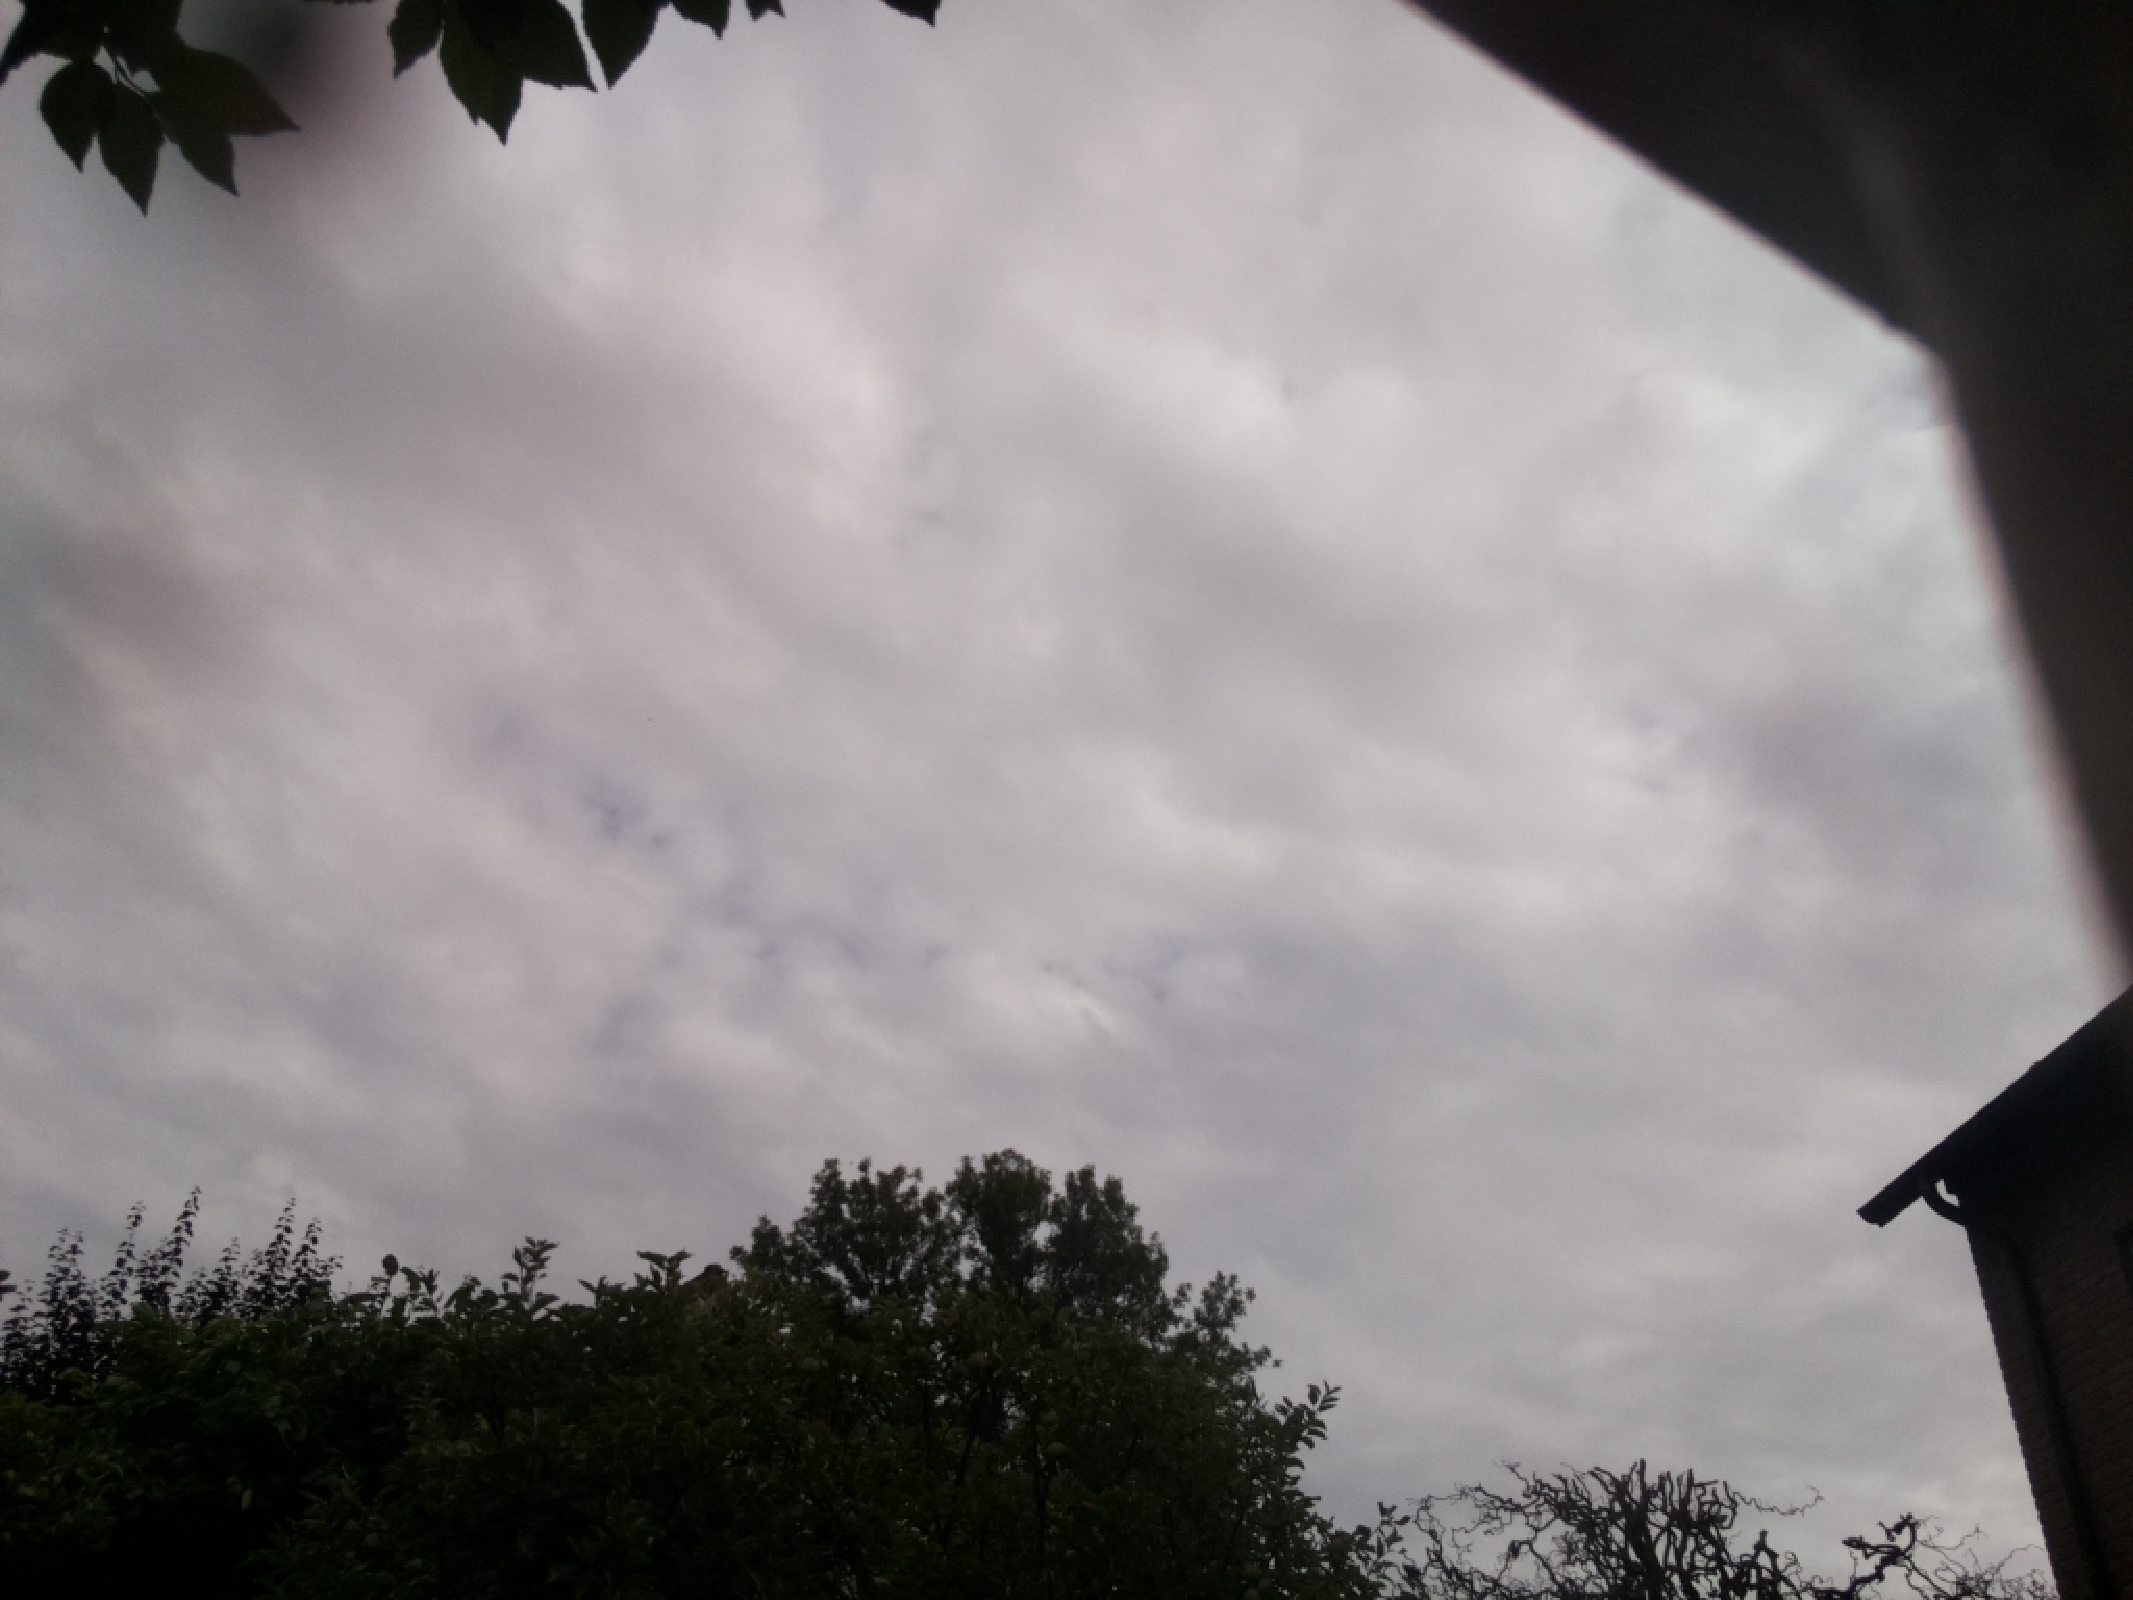
\includegraphics[width=\textwidth]{./pictures/cloudtypes/altostratus.pdf}
		\end{center}
		\caption{Altostratus}
		\label{fig:altocumulus}
		\end{subfigure}
		\begin{subfigure}[b]{0.31\textwidth}
		\begin{center}
				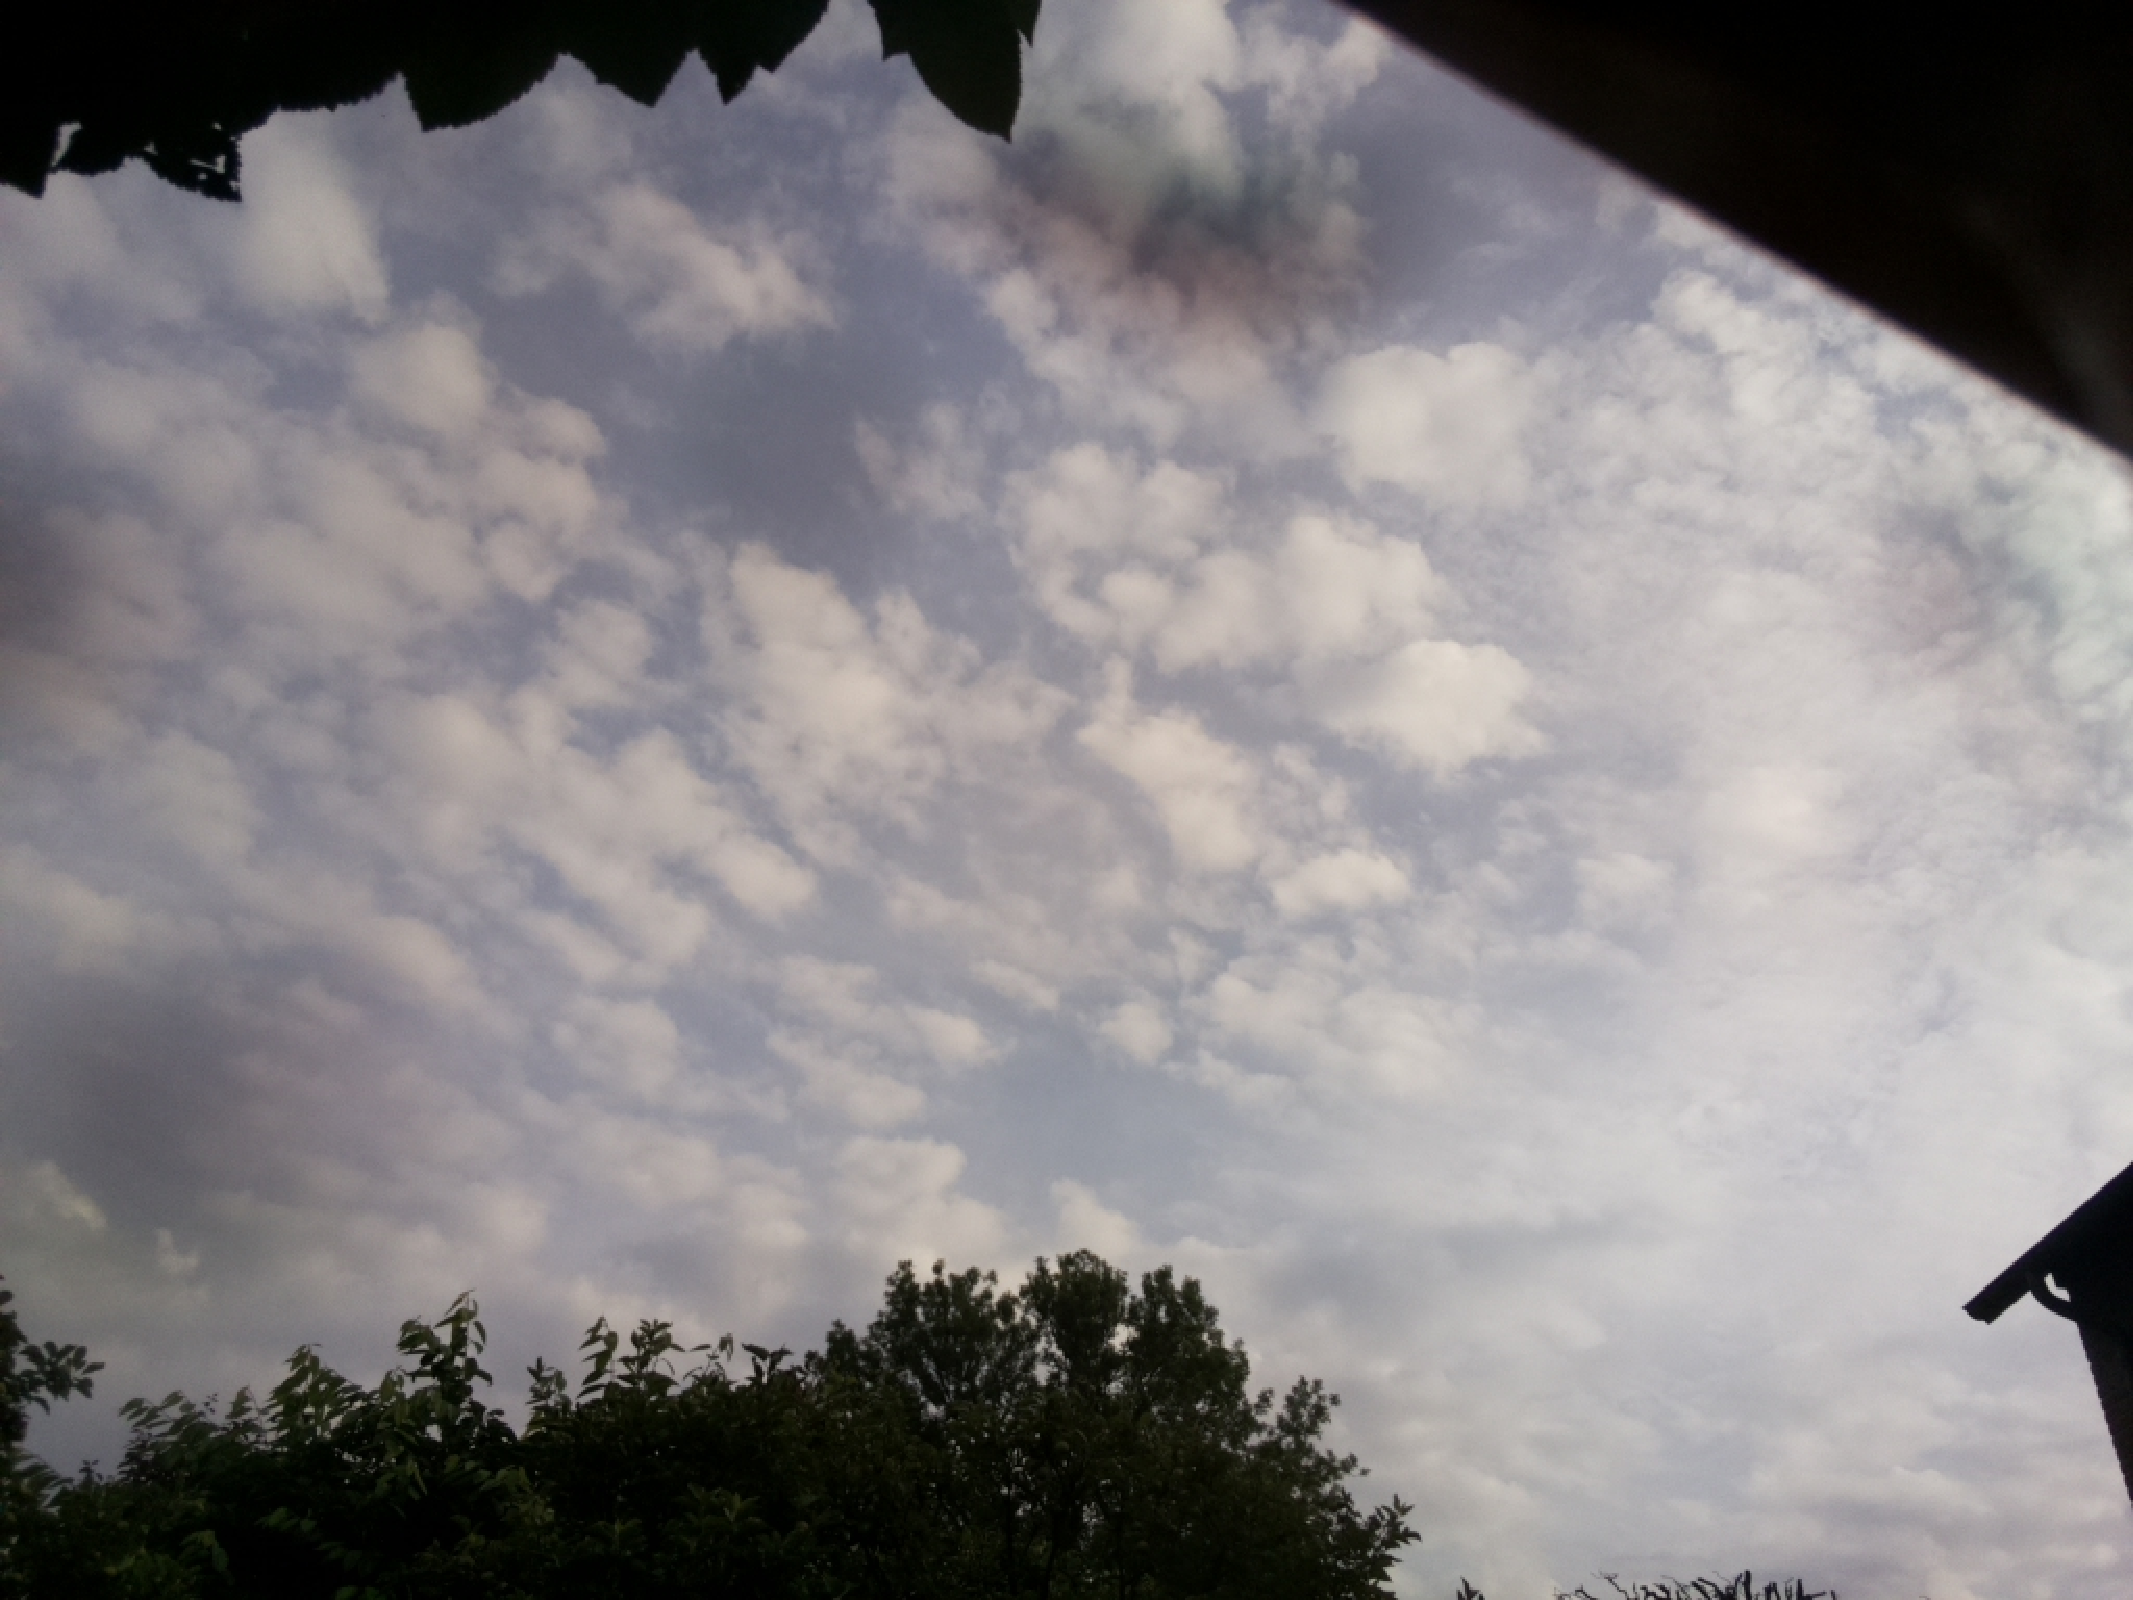
\includegraphics[width=\textwidth]{./pictures/cloudtypes/cirrocumulus.pdf}
		\end{center}
		\caption{Cirrocumulus}
		\label{fig:cirrocumulus}
		\end{subfigure}
		\begin{subfigure}[b]{0.31\textwidth}
		\begin{center}
				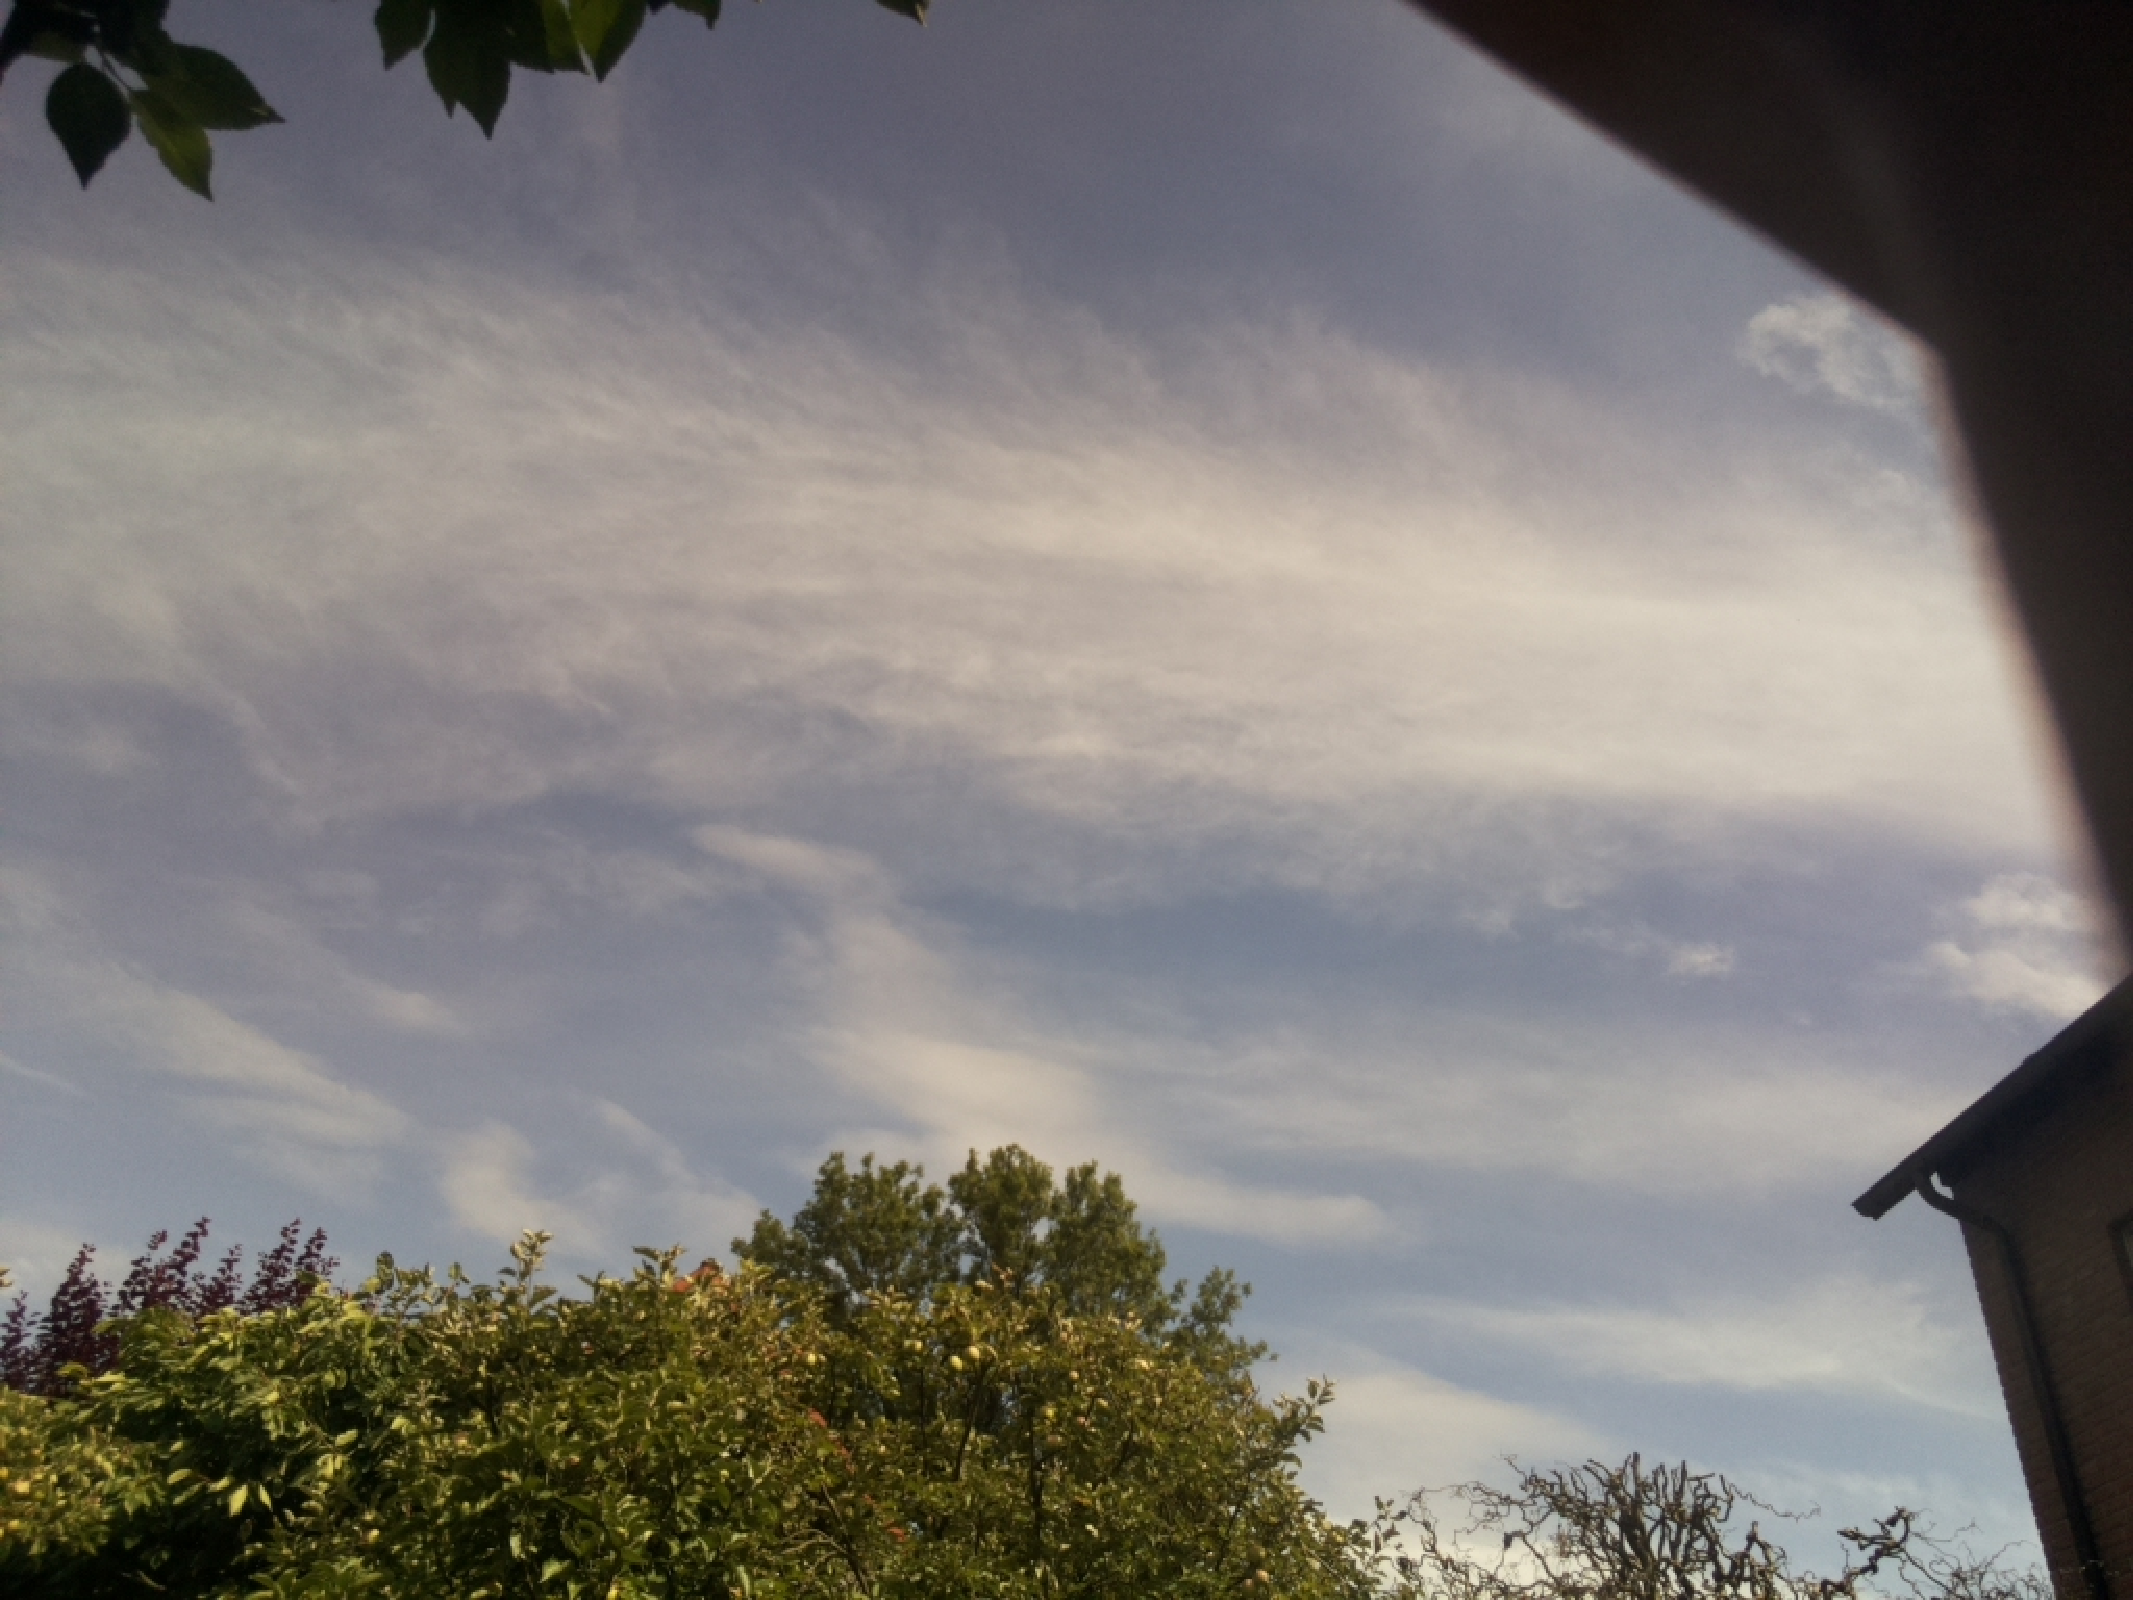
\includegraphics[width=\textwidth]{./pictures/cloudtypes/cirrostratus.pdf}
		\end{center}
		\caption{Cirrostratus}
		\label{fig:cirrostratus}
		\end{subfigure}
		\begin{subfigure}[b]{0.31\textwidth}
		\begin{center}
				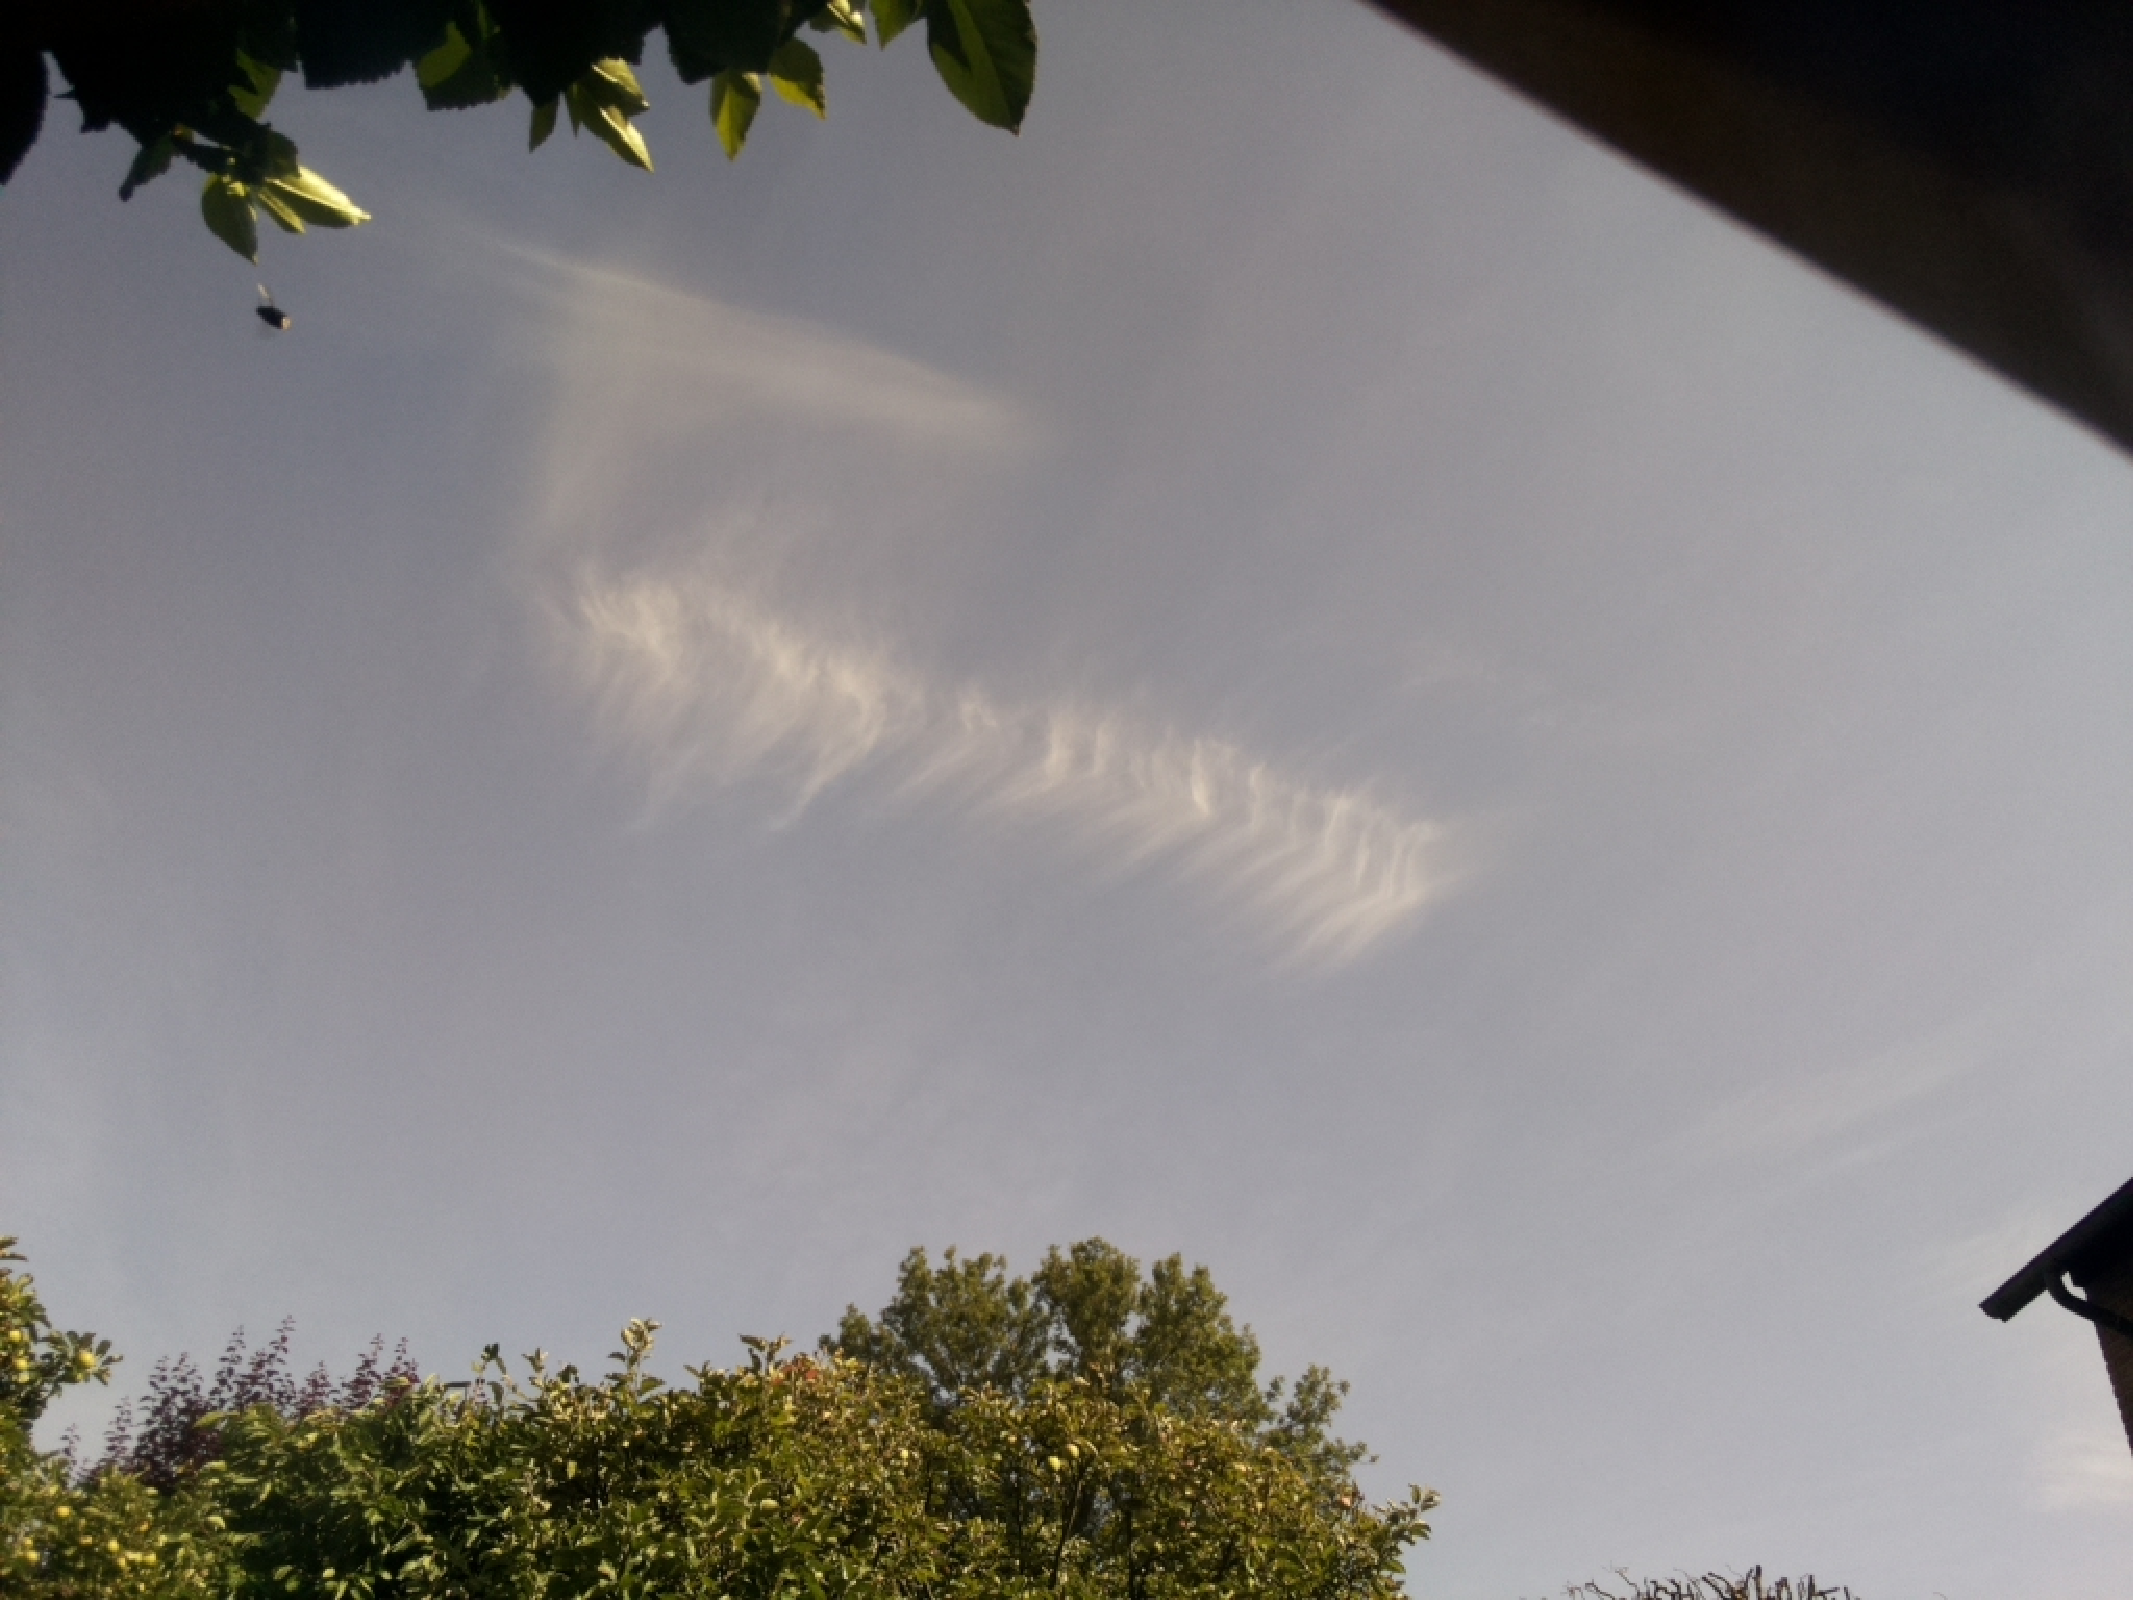
\includegraphics[width=\textwidth]{./pictures/cloudtypes/cirrus.pdf}
		\end{center}
		\caption{Cirrus}
		\label{fig:cirrus}
		\end{subfigure}
		\begin{subfigure}[b]{0.31\textwidth}
		\begin{center}
				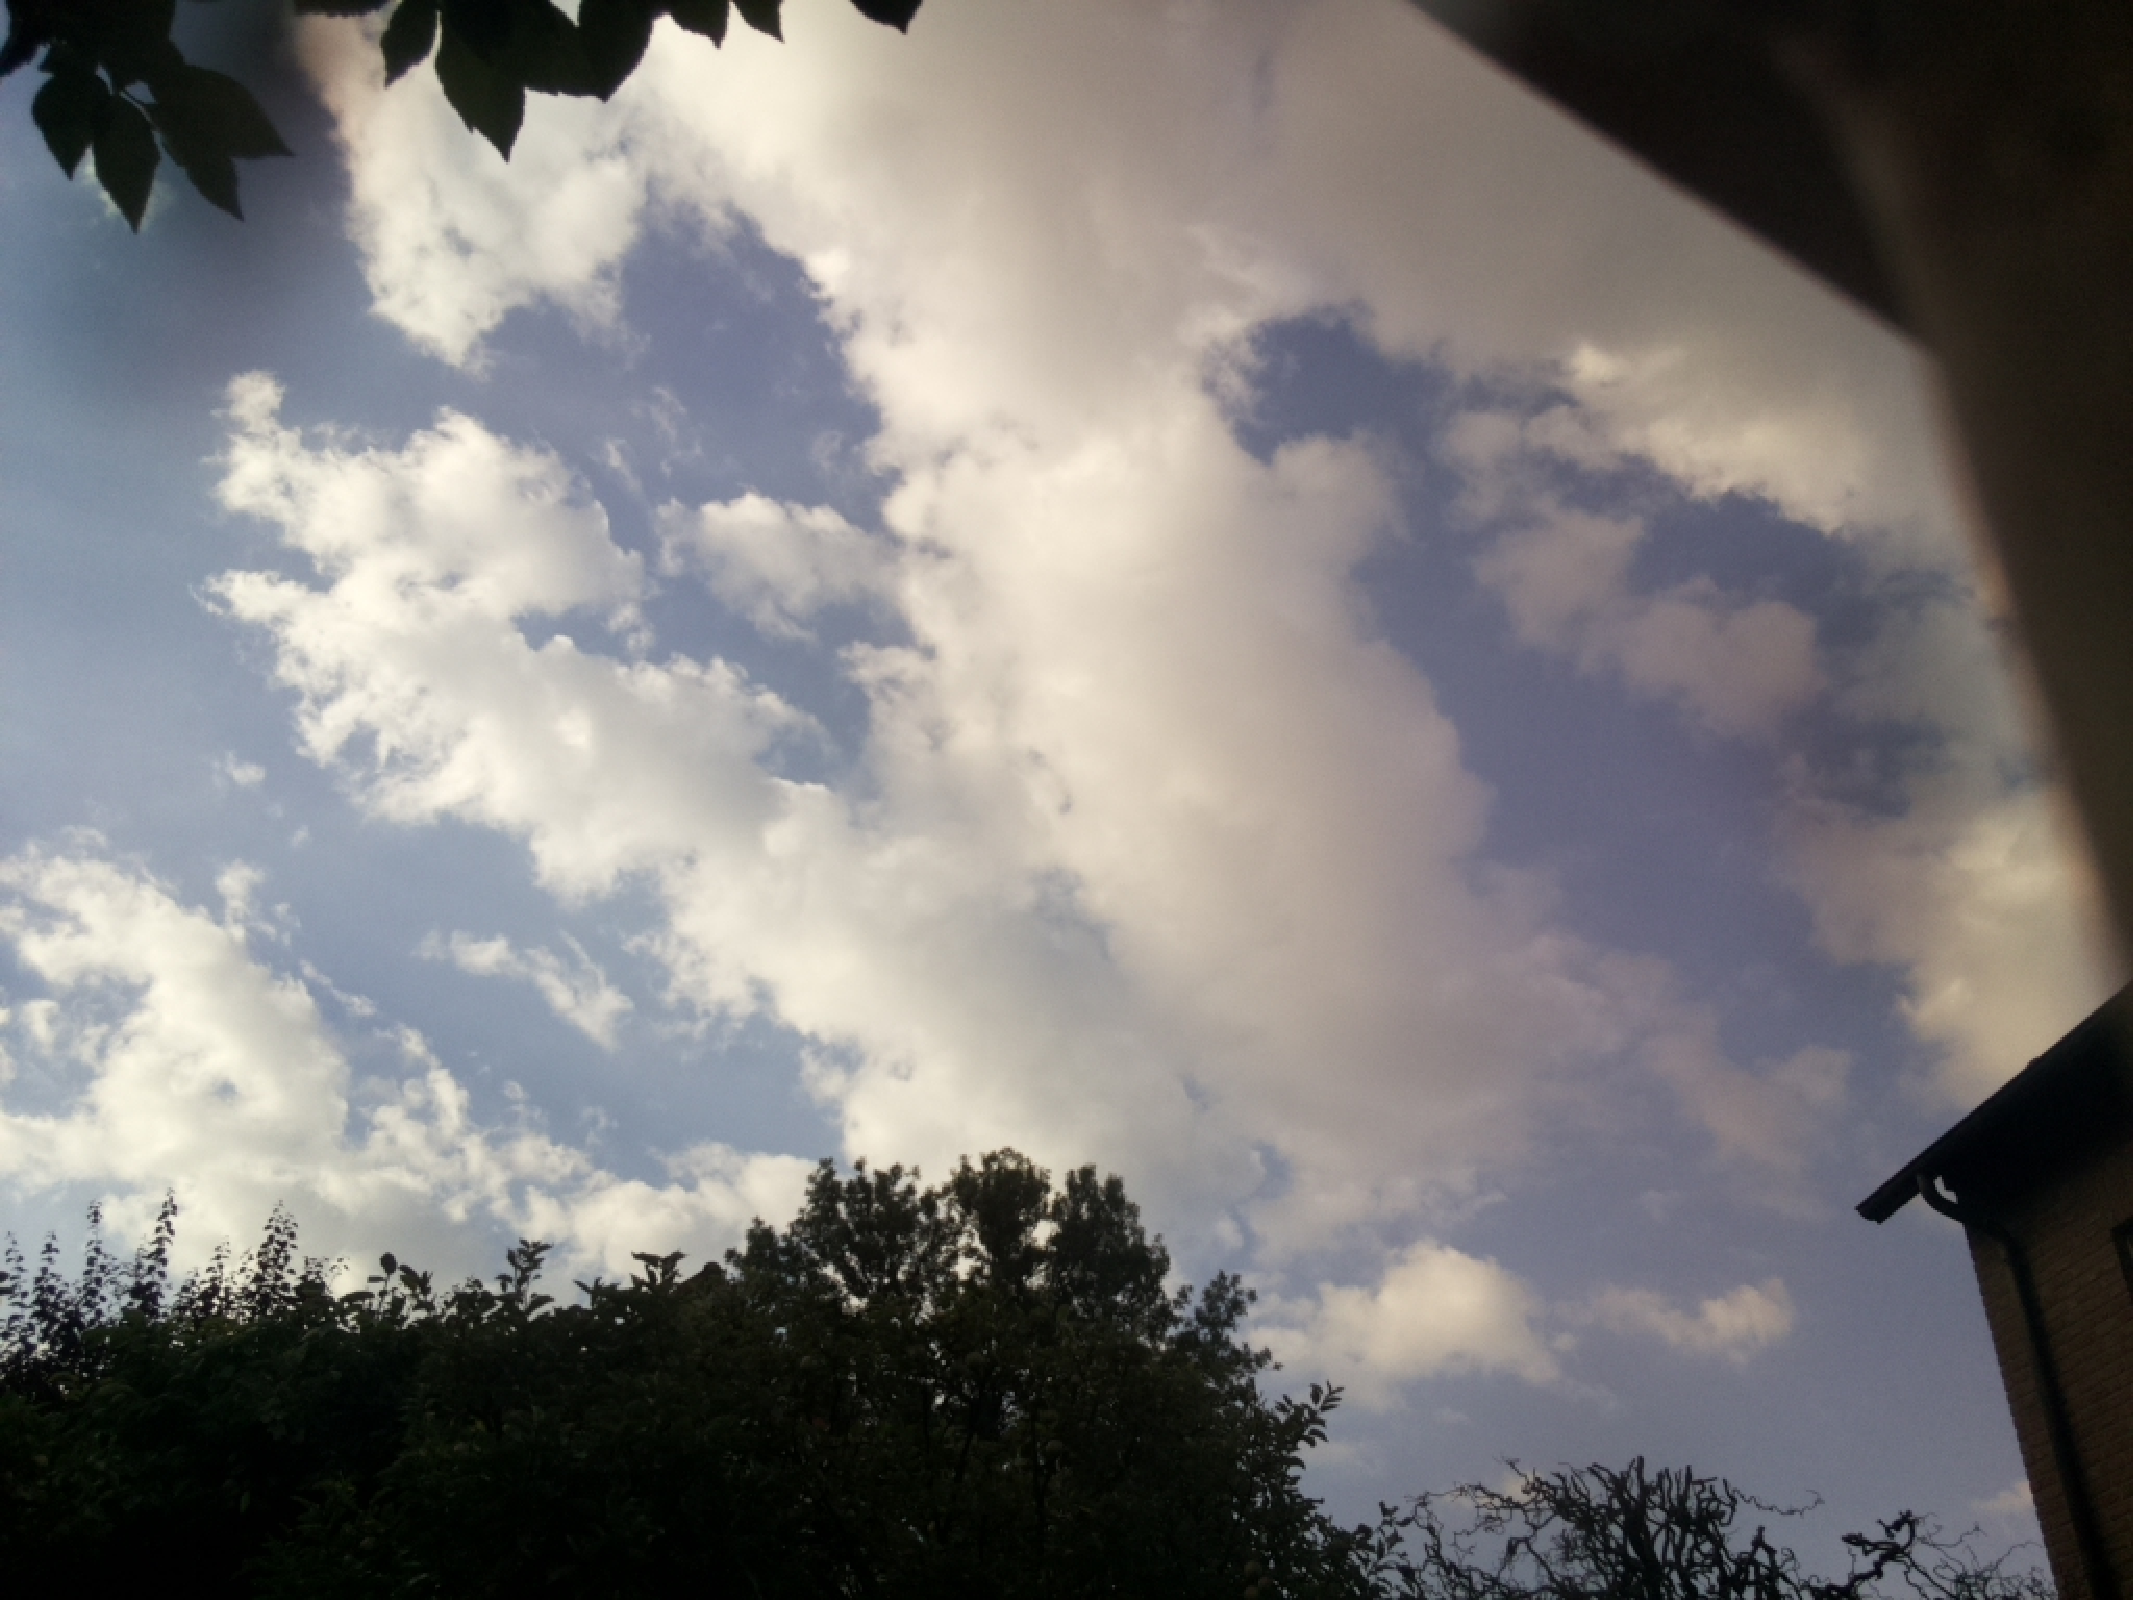
\includegraphics[width=\textwidth]{./pictures/cloudtypes/cumulus.pdf}
		\end{center}
		\caption{Cumulus}
		\label{fig:Cumulus}
		\end{subfigure}
		\begin{subfigure}[b]{0.31\textwidth}
		\begin{center}
				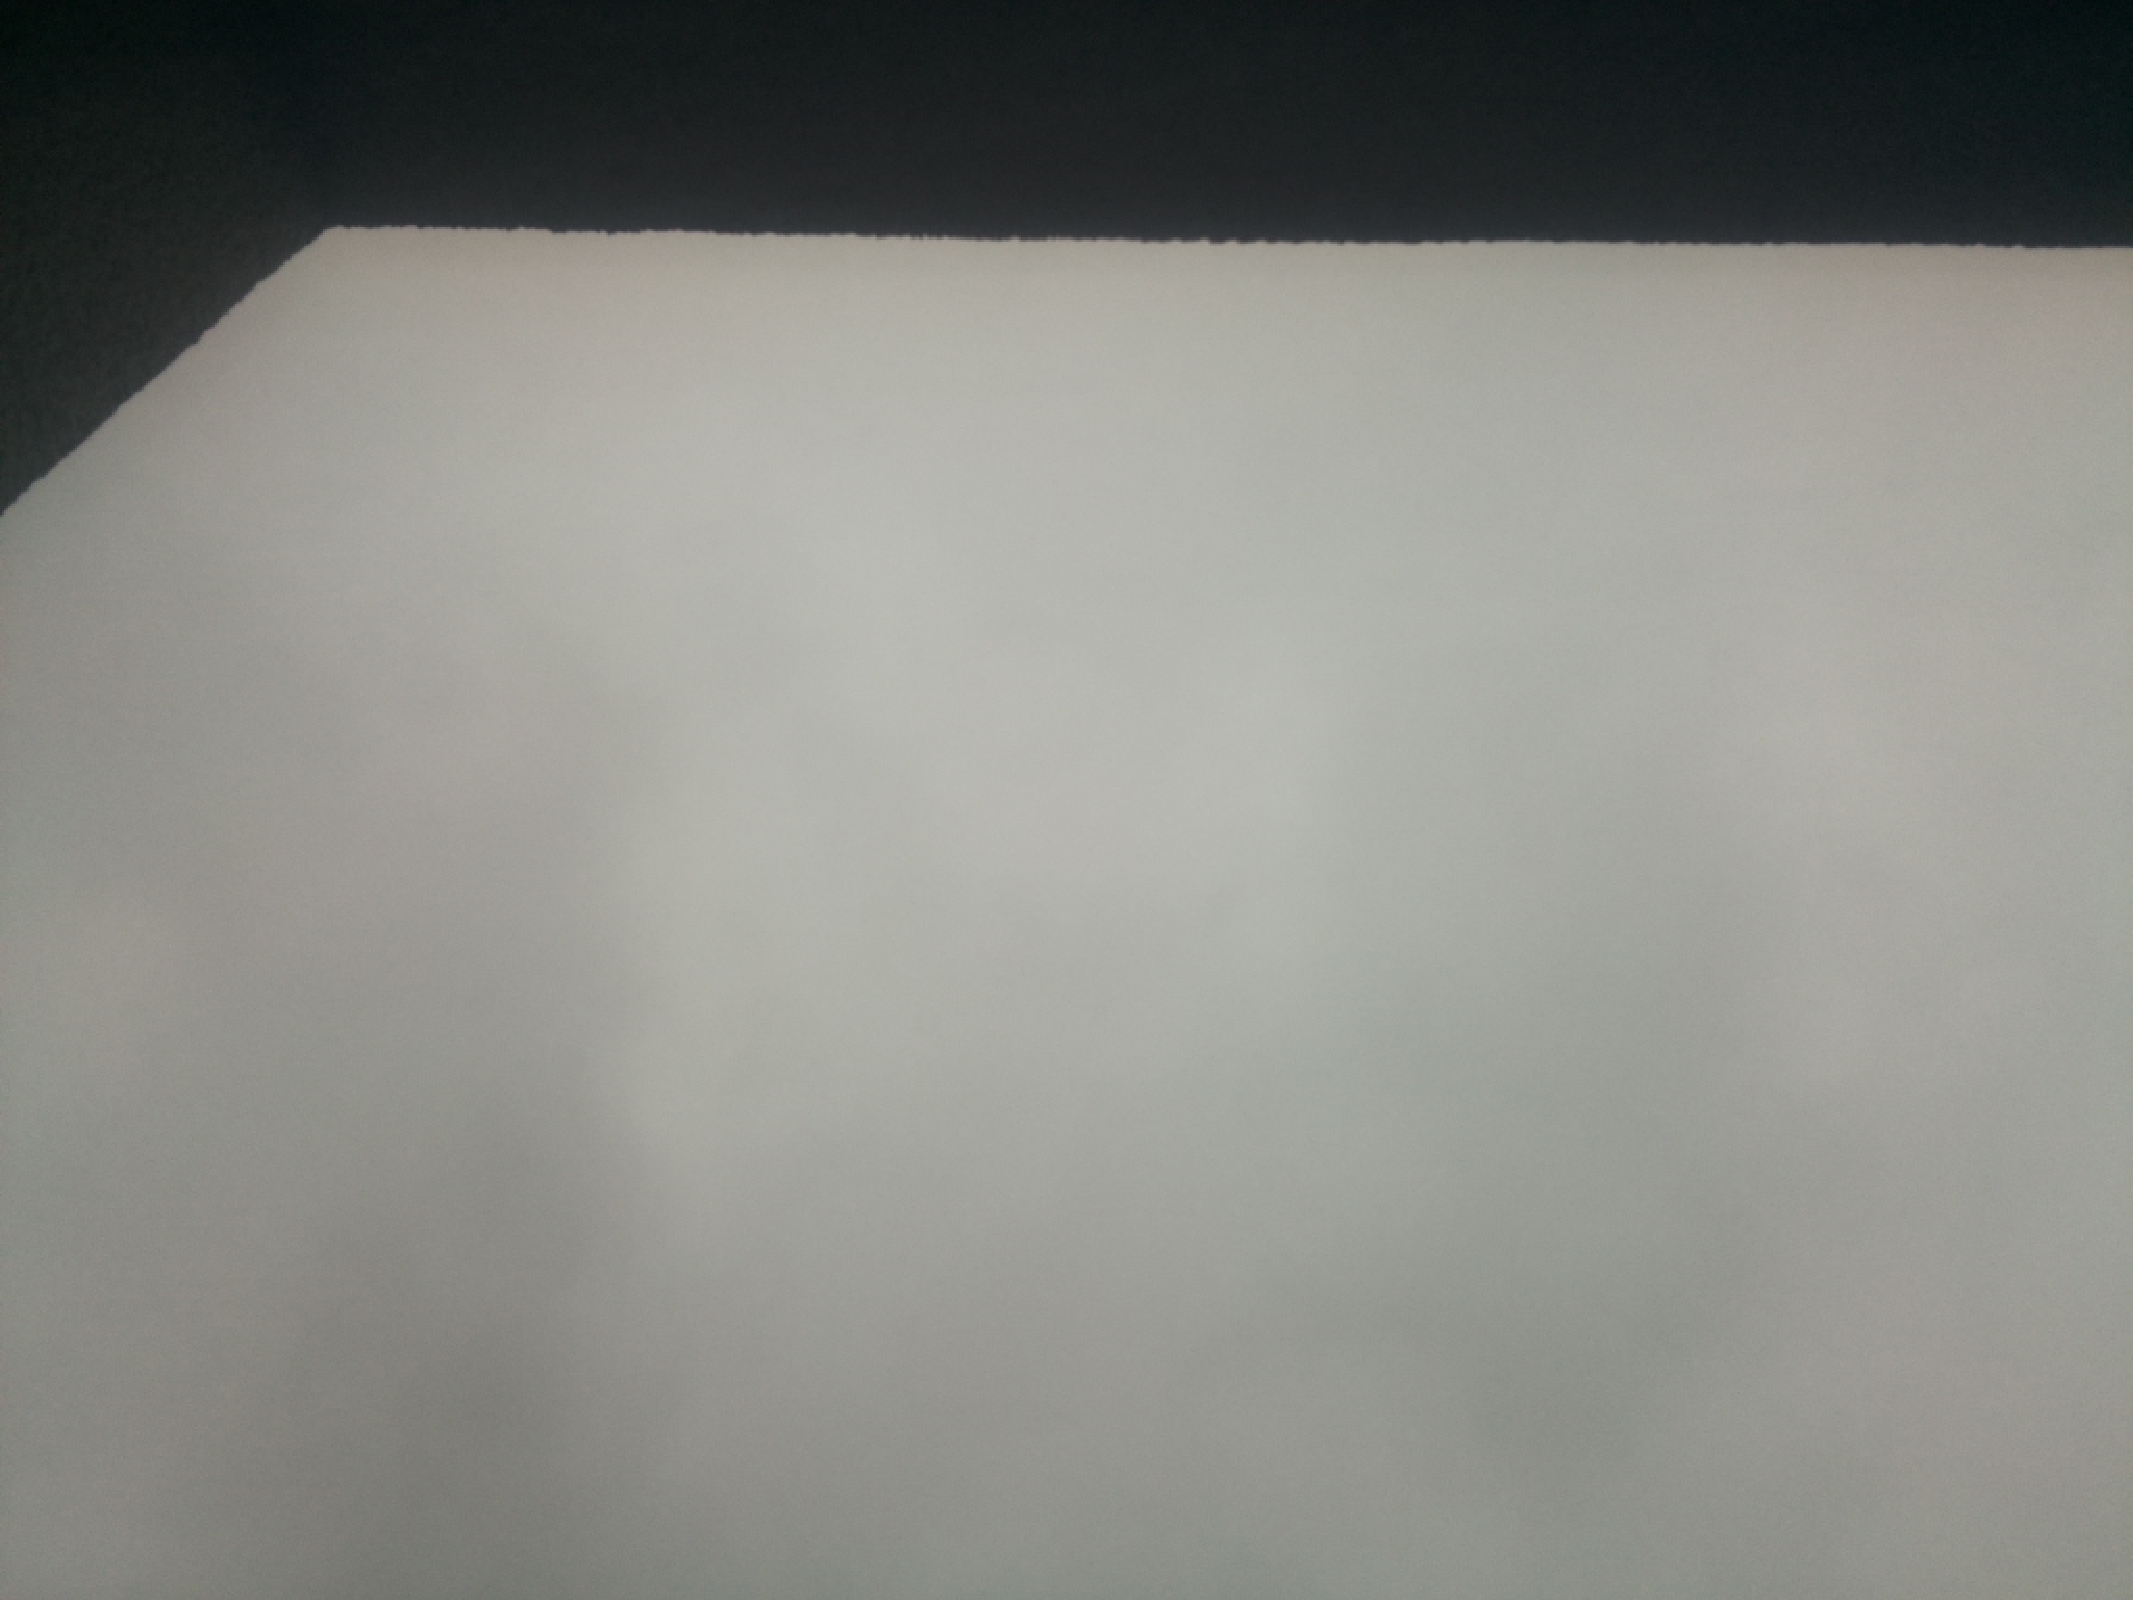
\includegraphics[width=\textwidth]{./pictures/cloudtypes/nimbostratus.pdf}
		\end{center}
		\caption{Nimbostratus}
		\label{fig:nimbostratus}
		\end{subfigure}
		\begin{subfigure}[b]{0.31\textwidth}
		\begin{center}
				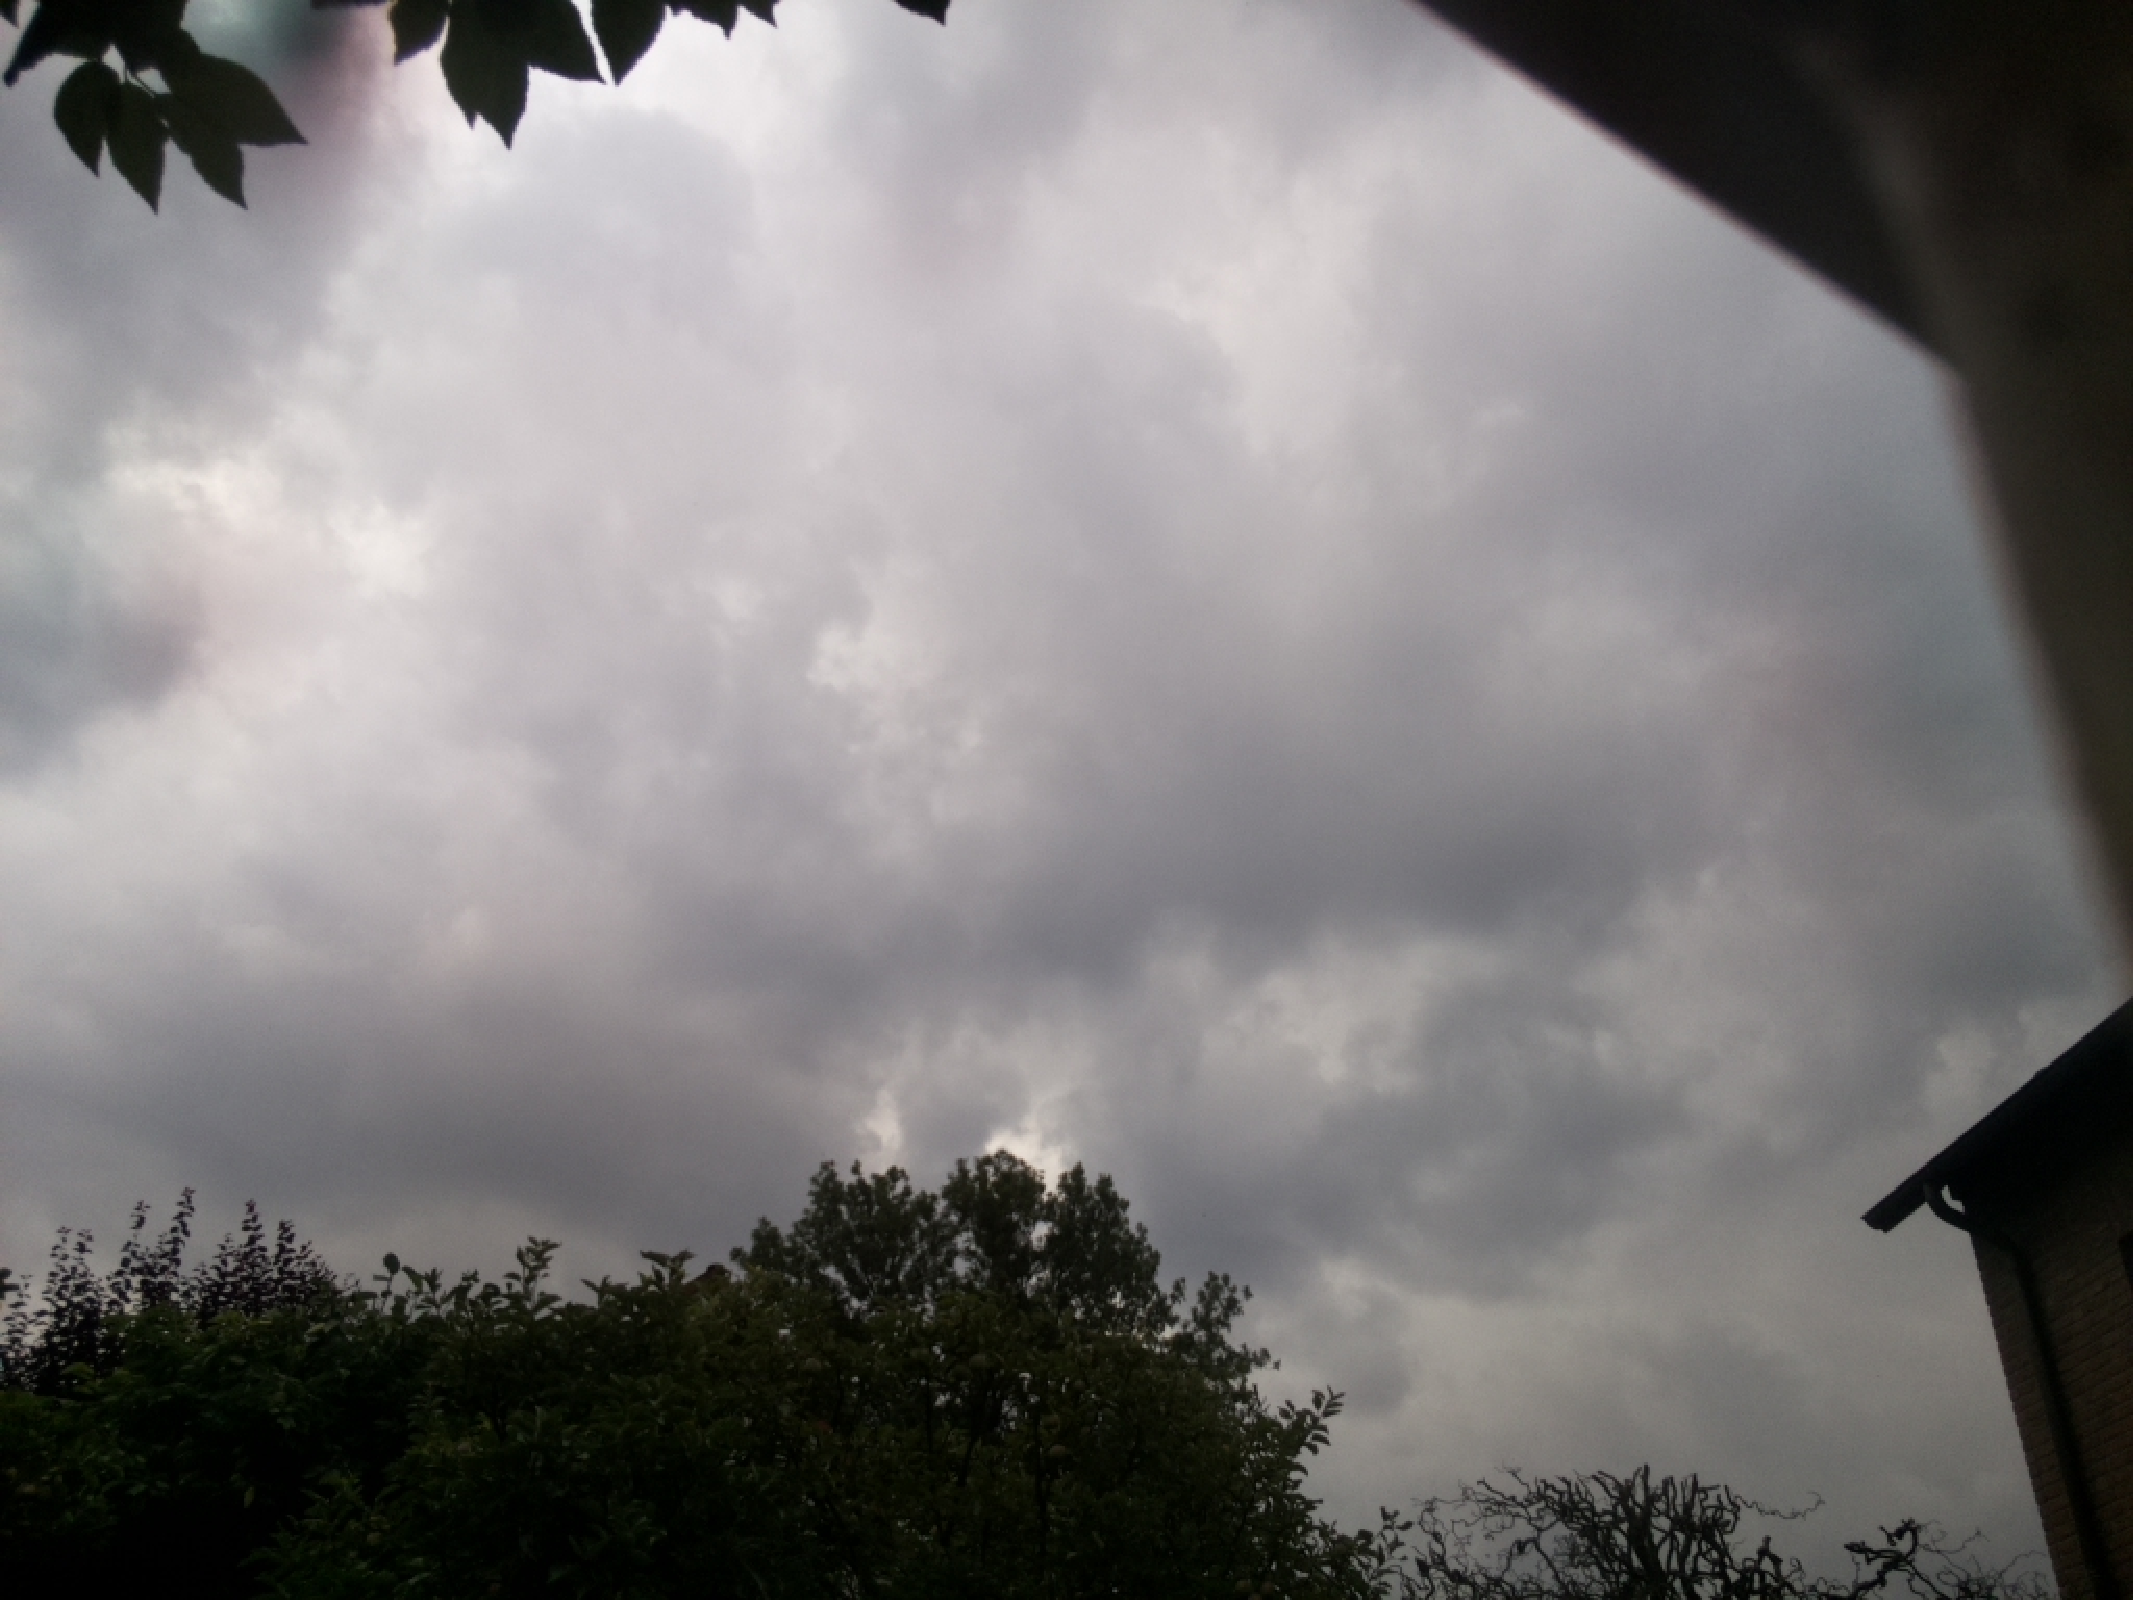
\includegraphics[width=\textwidth]{./pictures/cloudtypes/stratocumulus.pdf}
		\end{center}
		\caption{Stratocumulus}
		\label{fig:stratocumulus}
		\end{subfigure}
		\begin{subfigure}[b]{0.31\textwidth}
		\begin{center}
				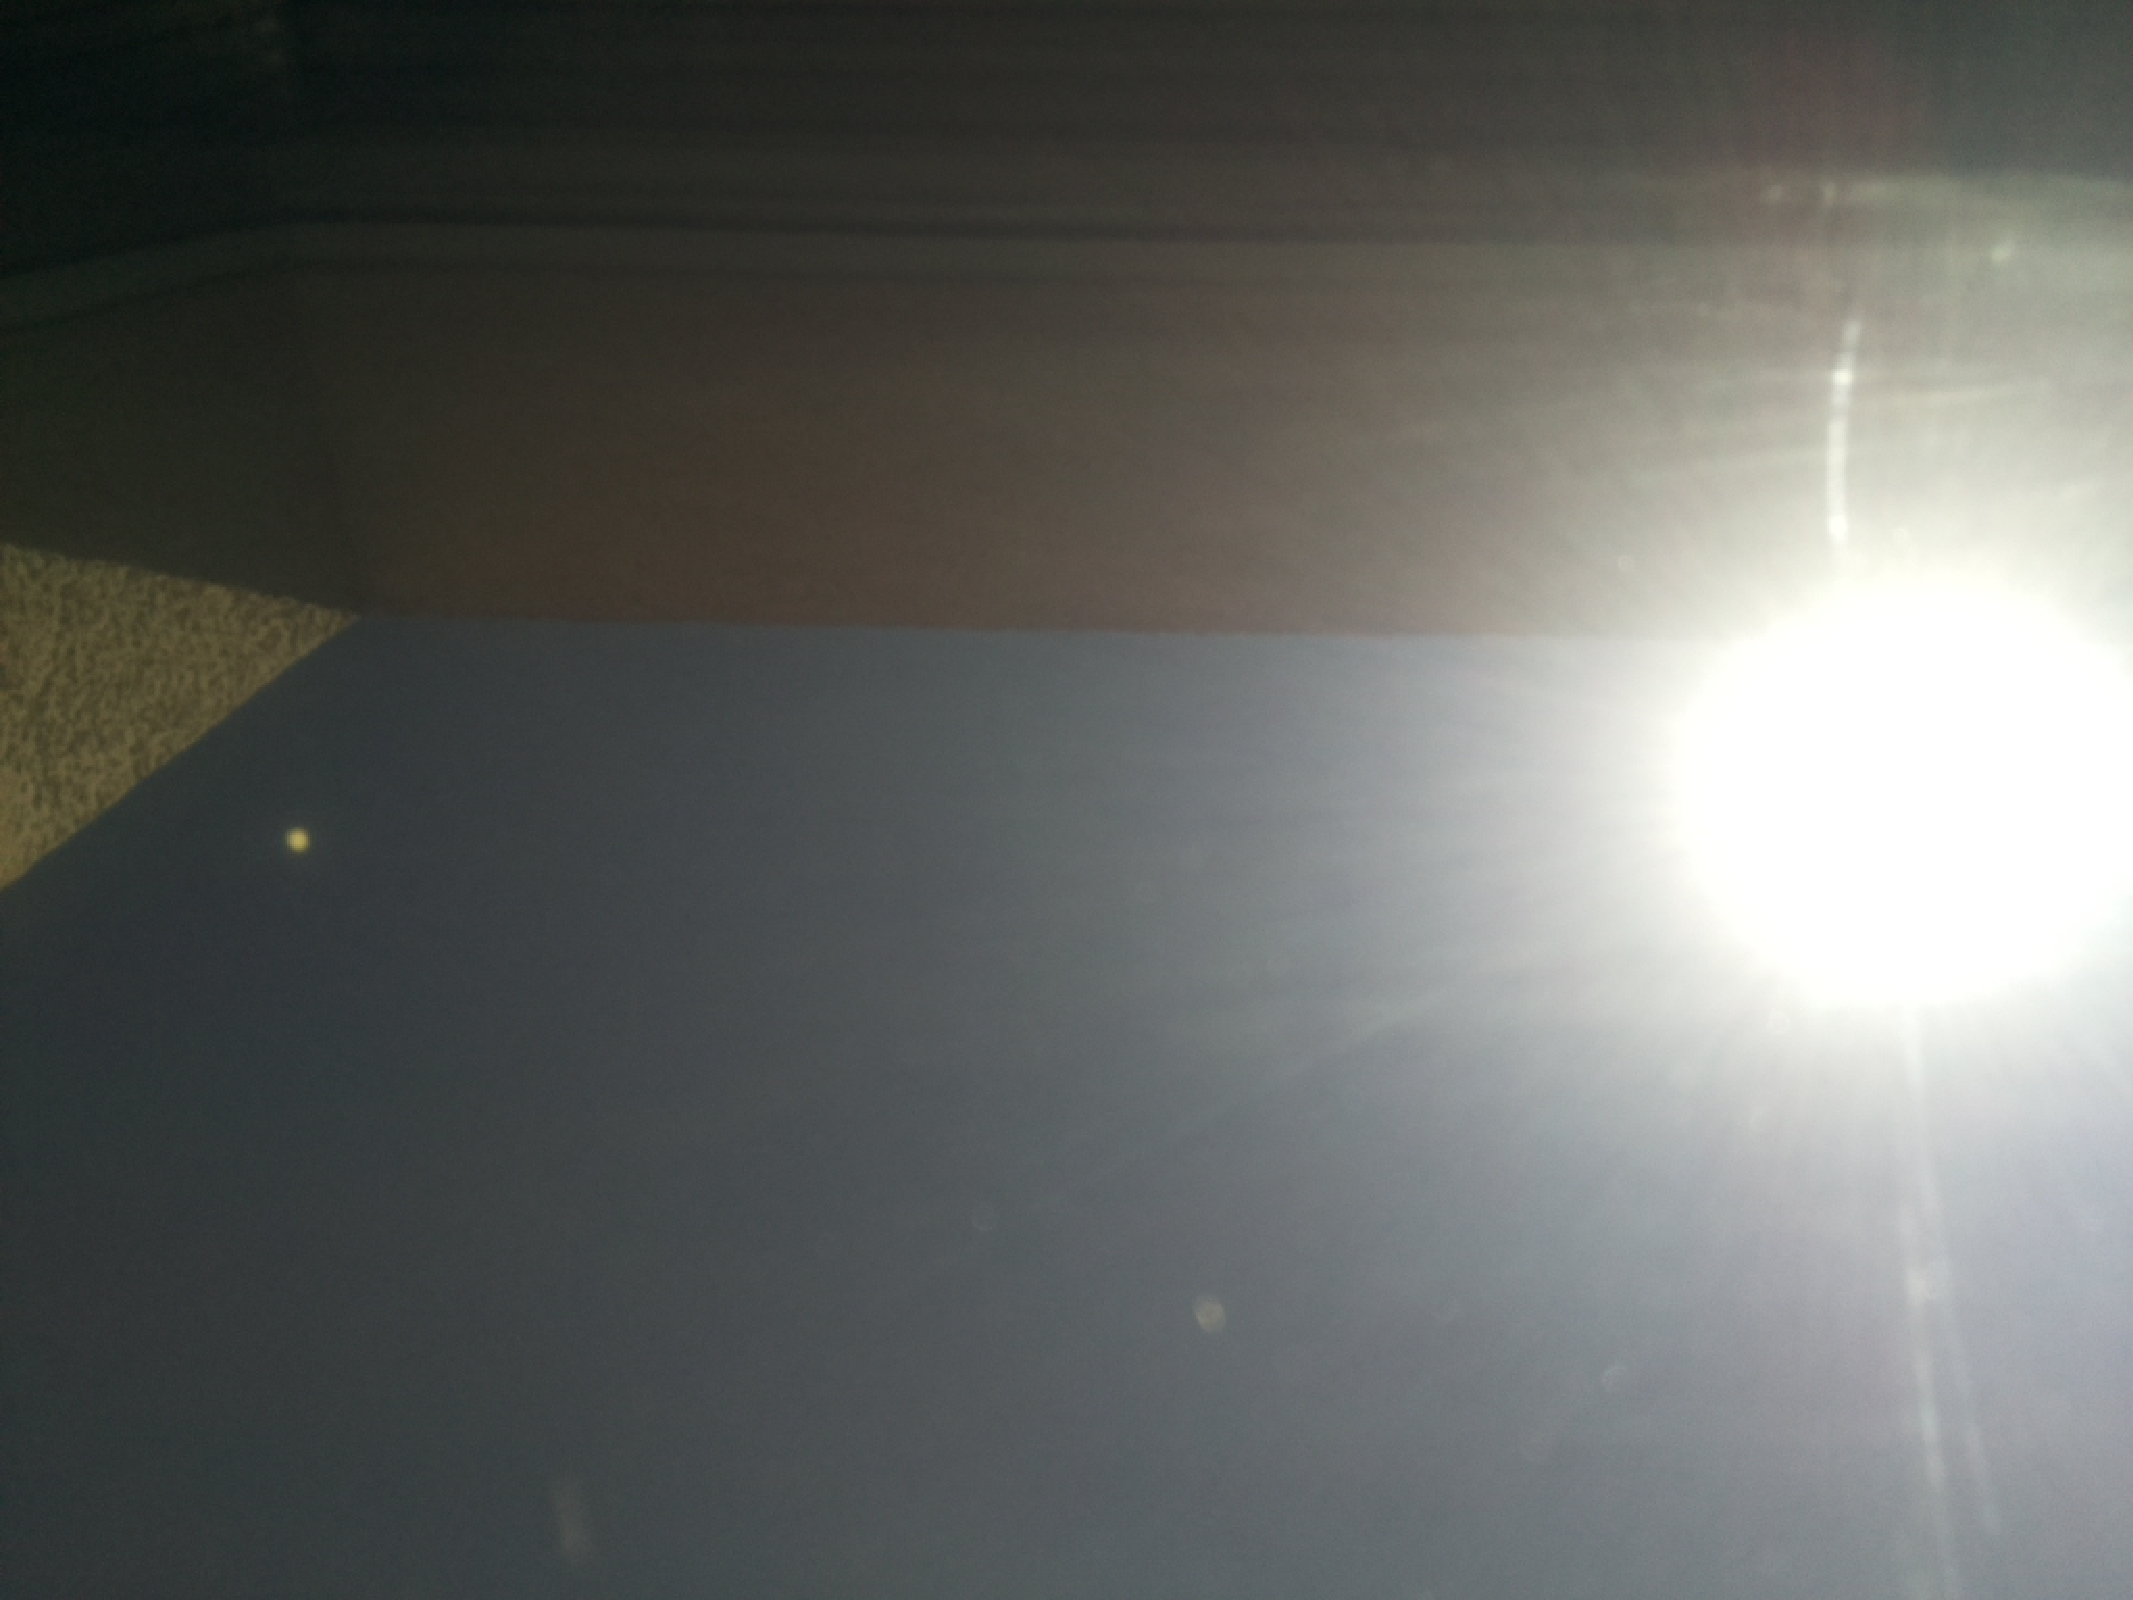
\includegraphics[width=\textwidth]{./pictures/cloudtypes/no_clouds.pdf}
		\end{center}
		\caption{keine Wolken}
		\label{fig:no_clouds}
		\end{subfigure}
		\caption{Representative Fotos fuer die unterschiedlichen Wolkenklassen.
		Dabei können die Wolkenformen stark variieren. Fuer umfassendere
		Information koennen bei dem
		\href{https://telegram.me/weatherpi_bot}{\texttt{TelegramBot}} unter dem
		Punkt \textit{label $\rightarrow$ label $\rightarrow$ info} weitere 
		Informationen angefordert werden.}
		\label{fig:}
\end{figure}
